% Manuscript prepared for submission to Nature Machine Intelligence.
% Single-column article-class format, structured as Introduction / Results /
% Discussion / Methods following Nature's research-article convention.
% Compiles with a standard TeX distribution (TeX Live) or tectonic.
\documentclass[11pt]{article}

\usepackage[a4paper,margin=1in]{geometry}
\usepackage{amsmath,amssymb,amsfonts,amsthm,mathtools}
\usepackage{bm}
\usepackage{graphicx}
\usepackage{booktabs}
\usepackage{float}
\usepackage{enumitem}
\usepackage[numbers,sort&compress]{natbib}
\usepackage{microtype}
\usepackage{xcolor}
\usepackage[colorlinks=true,linkcolor=blue,citecolor=blue,urlcolor=blue]{hyperref}

\graphicspath{{figures/}}

\newtheorem{theorem}{Theorem}
\newtheorem{lemma}[theorem]{Lemma}
\newtheorem{proposition}[theorem]{Proposition}
\newtheorem{corollary}[theorem]{Corollary}
\newtheorem{definition}{Definition}
\newtheorem{remark}{Remark}

\DeclareMathOperator{\Tr}{Tr}
\newcommand{\R}{\mathbb{R}}
\newcommand{\F}{\mathbb{F}}
\newcommand{\calD}{\mathcal{D}}
\newcommand{\calS}{\mathcal{S}}
\newcommand{\calG}{\mathcal{G}}
\newcommand{\eps}{\varepsilon}
\newcommand{\abs}[1]{\left\lvert #1 \right\rvert}
% \sync{...} marks numbers read directly from the regenerated summary.json /
% tables; it is the identity so the value appears verbatim.
\newcommand{\sync}[1]{#1}

\title{\bfseries Selective and Calibrated Decoding for Quantum Error Correction:\\
A Topology-Aware Decoder-Family Benchmark under Structured Noise}

\author{Molena Huynh\\[3pt]
\normalsize [Affiliation to be completed before submission]}

\date{\today}

\begin{document}

\maketitle

\begin{abstract}
A quantum error-correcting code only protects information if its \emph{decoder} maps a measured syndrome to the right recovery---quickly, and under the \emph{structured} noise that real hardware exhibits: bias, spatial bursts, neighbour correlations and faulty syndrome read-out. Most decoder studies optimise a single number, the logical error rate, and report it under independent-and-identically-distributed (i.i.d.) noise. We argue that two further axes are at least as important for deployable decoding and are usually treated as afterthoughts: the ability to \emph{abstain} when a decoder is unsure (selective decoding), and the \emph{calibration} of the confidence that drives such abstention. We build a unified, reproducible benchmark that evaluates a full decoder family---an optimal lookup leader, majority vote, minimum-weight matching, belief propagation, a learned neural coset selector, a topology-feature decoder, a confidence-fused decoder, and a reinforcement-learning (contextual-bandit) selector---across five structured-noise regimes on a distance-$d$ repetition code, treating logical error rate, expected calibration error (ECE) and the risk--coverage trade-off as first-class metrics with analytic 95\% confidence intervals. At reported scale (distance $9$, $40{,}000$ trials per regime, $200{,}000$ pooled shots per decoder), our central, deliberately conservative finding is that the decoders are \emph{statistically indistinguishable} on raw logical error rate (means \sync{0.1516}--\sync{0.1540}, 95\% confidence intervals $\approx\pm\sync{0.0016}$; the best-to-worst spread of $\sync{0.0024}$ is below one full interval width), so claims of one decoder ``beating'' another are not supported by the data. The genuine, separable contributions live elsewhere: (i)~a framework and audit discipline that compares the whole decoder family under structured noise on a single defect-graph interface; (ii)~abstention, which under selective decoding drives matching's committed logical error from \sync{0.1529} at full coverage down to \sync{0.0758} at \sync{0.55} coverage and \sync{0.0099} at \sync{0.25} coverage; and (iii)~calibration, where ECE varies eight-fold across decoders and is uncorrelated with sophistication---the lowest ECE belongs to the lightweight \emph{neural} coset selector (\sync{0.0317}), while plain minimum-weight \emph{matching} is the worst calibrated (\sync{0.2608}). Notably, this contradicts a natural intuition (and a claim in the project's own README) that the fused decoder is best calibrated; we report the artifact's numbers, not the intuition. We frame the work as a calibrated, selective-decoding benchmark, not a superiority claim.
\end{abstract}

% ============================================================
\section{Introduction}
\label{sec:introduction}

Quantum error correction (QEC) protects logical information by encoding it redundantly across many physical qubits and repeatedly measuring stabilizer operators, whose outcomes form a \emph{syndrome}~\cite{shor1995scheme,nielsen2010quantum,terhal2015quantum}. Topological codes---most prominently Kitaev's toric and surface codes~\cite{kitaev2003fault,dennis2002topological,fowler2012surface}---are the leading candidates for scalable fault tolerance, and recent hardware has demonstrated that scaling such a code can suppress the logical error rate below the physical one~\cite{google2023suppressing}. The component that turns a syndrome into a correction is the \emph{decoder}, and it is the part of the stack where classical algorithms and, increasingly, machine learning meet the physics of the device.

The dominant decoder for surface codes is minimum-weight perfect matching (MWPM)~\cite{dennis2002topological,fowler2012surface,higgott2022pymatching}, built on Edmonds' blossom algorithm~\cite{edmonds1965paths}; belief propagation (BP) and BP with ordered-statistics decoding underpin quantum low-density-parity-check decoding~\cite{poulin2008iterative,panteleev2021degenerate,roffe2020decoding}. A large and growing literature applies neural networks and reinforcement learning to decoding~\cite{torlai2017neural,varsamopoulos2017decoding,baireuther2018machine,krastanov2017deep,sweke2020reinforcement,andreasson2019quantum}, and very recent work demonstrates learned decoders that exceed matching-based accuracy on real hardware syndromes~\cite{bausch2024learning}. The headline metric in nearly all of this work is the logical error rate, almost always evaluated under i.i.d.\ (depolarizing or bit-flip) noise.

Two facts motivate this paper. First, hardware noise is not i.i.d. It is \emph{structured}: dominated by one Pauli type (bias), spatially bursty, correlated between neighbours, and accompanied by faulty syndrome extraction. A decoder that is excellent on i.i.d.\ noise may or may not retain its advantage under structure, and the only way to know is to test the same decoder family across regimes on one footing. Second, a decoder that runs inside a fault-tolerant control loop does not have to commit to every syndrome. It can \emph{abstain}---flagging a shot as unreliable so that a slower fallback decoder, a repeated measurement, or a higher-level protocol takes over. Abstention is the QEC analogue of \emph{selective prediction} in machine learning~\cite{chow1970optimum,elyaniv2010foundations,geifman2017selective}, and it is only useful if the confidence that gates it is \emph{calibrated}~\cite{guo2017calibration,naeini2015obtaining}. These two axes---coverage and calibration---are routinely omitted from decoder benchmarks.

\paragraph{This work.}
We treat decoding as a problem on the code's \emph{defect graph} and build a unified, fully reproducible benchmark with three properties usually kept separate. (1)~\emph{Breadth}: a single \texttt{decode(syndrome)$\,\to\,$(correction, confidence)} interface hosts eight decoders spanning the textbook-to-learned spectrum, evaluated across five structured-noise regimes. (2)~\emph{Selectivity}: every decoder can abstain, so we report risk--coverage curves, not just a single error rate. (3)~\emph{Calibration}: expected calibration error is a first-class output alongside the logical error rate, with analytic 95\% confidence intervals so that statistical significance is visible rather than assumed.

\paragraph{What we claim, and what we do not.}
We are deliberately conservative. On the repetition code and the regimes we study, at reported scale the eight decoders' logical error rates lie within each other's confidence intervals (Sec.~\ref{sec:headline}); we therefore do \emph{not} claim that any decoder beats another on raw accuracy, and we say so explicitly. What the benchmark does establish is (i)~that abstention buys a large, monotone reduction in committed logical error---matching's committed risk falls from \sync{0.1529} at full coverage to \sync{0.0758} at \sync{0.55} coverage and \sync{0.0099} at \sync{0.25} coverage (Sec.~\ref{sec:risk_coverage})---and (ii)~that calibration quality is \emph{not} predicted by decoder sophistication: ECE ranges from \sync{0.0317} (the lightweight neural coset selector) to \sync{0.2608} (plain minimum-weight matching), an eight-fold spread with no monotone relationship to decoder complexity. The contribution is the framework, the selective/calibrated lens, and the honest accounting---not a new state-of-the-art error rate. This audit ethos is enforced in code: a readiness gate rejects any reported number that does not trace to a generated artifact and rejects forbidden absolute-superiority phrasing.

\subsection{Contributions}
\label{sec:contributions}
\begin{enumerate}[leftmargin=1.5em]
    \item \textbf{A decoder-family benchmark under structured noise.} Eight decoders (lookup, majority, matching, BP, neural, topology, fused, RL selector) on one defect-graph interface, evaluated across i.i.d., biased, burst, correlated, and measurement-error regimes, with per-regime breakdowns and threshold curves.
    \item \textbf{Selective decoding as a primary axis.} Confidence-gated abstention and risk--coverage curves for every decoder, quantifying the reliability bought by giving up coverage.
    \item \textbf{Calibration as a first-class metric.} Expected calibration error reported for all decoders with 95\% confidence intervals, exposing that calibration is uncorrelated with decoder complexity.
    \item \textbf{An honest, reproducible accounting.} A single source-of-truth artifact, analytic confidence intervals that reveal the decoders to be statistically indistinguishable on raw logical error, and a code-level audit gate against fabricated numbers and superiority claims.
\end{enumerate}

% ============================================================
\subsection{Theory: selective decoding risk}
\label{sec:selective_theory}

The risk--coverage view has a simple decision-theoretic guarantee when the
confidence score is calibrated and monotone in the conditional success
probability. This is the formal reason calibration is reported alongside error
rate.

\begin{theorem}[Monotone selective risk under calibrated confidence]
\label{thm:selective-risk}
Let $F\in\{0,1\}$ be the logical-failure indicator for a decoder and let
$C\in[0,1]$ be a confidence score such that
$\Pr(F=0\mid C=c)=c$ almost surely. For a threshold $\tau$ with
$\Pr(C\ge\tau)>0$, define committed risk
$R(\tau)=\Pr(F=1\mid C\ge\tau)$. Then
$R(\tau)=1-\mathbb{E}[C\mid C\ge\tau]$ and $R(\tau)$ is non-increasing as
$\tau$ increases.
\end{theorem}

\begin{proof}
By calibration, $\Pr(F=1\mid C)=1-C$. Conditioning on $C\ge\tau$ and using the
tower property gives
$R(\tau)=\mathbb{E}[\Pr(F=1\mid C)\mid C\ge\tau]=1-\mathbb{E}[C\mid C\ge\tau]$.
If $\tau_2>\tau_1$, the conditional distribution under $C\ge\tau_2$ is the upper
tail of the distribution under $C\ge\tau_1$, so its conditional mean cannot be
smaller. Hence $R(\tau_2)\le R(\tau_1)$.
\end{proof}

The theorem is not assumed in the experiments; the empirical confidence scores
are imperfect, so the risk--coverage curves and ECE quantify how far each
decoder is from this ideal selective-decoding behaviour.

The results are stated conservatively. They are produced on small, fully reproducible simulated benchmarks (a repetition code and a surface-like toy lattice) under simulated structured noise; they are not hardware syndromes, not a full surface code at scale, and not a claim of superiority over production decoders. Those are future targets, not present facts (Sec.~\ref{sec:limitations}).

% ============================================================
\section{Results}
\label{sec:results}

\begin{figure}[t]
    \centering
    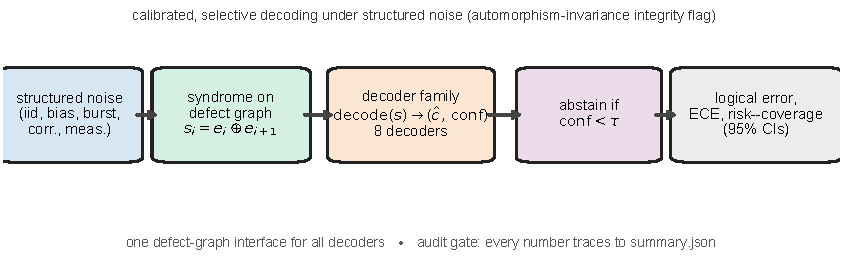
\includegraphics[width=\textwidth]{fig_schematic.pdf}
    \caption{\textbf{Overview of the selective, calibrated decoding benchmark.} A code word is corrupted by one of five structured-noise regimes (i.i.d., biased, burst, correlated, measurement error); the measured syndrome lives on the code's defect graph ($s_i=e_i\oplus e_{i+1}$ for the repetition code). A single \texttt{decode(syndrome)$\to$(correction, confidence)} interface hosts the whole eight-decoder family (lookup, majority, matching, BP, neural, topology, fused, RL selector), so every decoder is compared on one footing. A confidence threshold $\tau$ gates abstention (selective decoding), and three first-class metrics---logical error rate, expected calibration error, and the full risk--coverage curve---are scored with analytic $95\%$ confidence intervals. Two integrity guarantees underpin the benchmark: all decoders share one defect-graph interface, and an audit gate requires every reported number to trace to the single source-of-truth artifact \texttt{summary.json}, with an automorphism-invariance flag confirming the code's cyclic symmetry is respected.}
    \label{fig:schematic}
\end{figure}

\subsection{Benchmark design}
\label{sec:design}

Figure~\ref{fig:schematic} summarizes the end-to-end pipeline: structured noise corrupts a code word, the resulting syndrome on the defect graph is passed to the shared decoder interface, a confidence threshold gates abstention, and the logical error rate, calibration and risk--coverage metrics are scored with $95\%$ confidence intervals.

\paragraph{Codes and defect graphs.}
The primary benchmark is the bit-flip repetition code: $d$ data bits over $\F_2$ with $d-1$ weight-two parity checks $Z_iZ_{i+1}$. A syndrome bit $s_i=e_i\oplus e_{i+1}$ fires where an error chain crosses link $i$, so defects live on a one-dimensional line and decoding is a matching/pairing problem on that line. The single logical observable is the global parity, and a correction succeeds iff the residual $e\oplus \hat c$ is a stabilizer (trivial coset). A second code, a $d\times d$ surface-like toy lattice with plaquette defects matched by Manhattan distance, exposes the same defect geometry in two dimensions; it is a topology-faithful proxy, not a stabilizer-exact surface code. Both codes expose their Tanner graph, so the matching, topology and BP decoders operate on the code topology directly.

\paragraph{Structured-noise regimes.}
Five seeded samplers define the regimes (Methods, Sec.~\ref{sec:methods_noise}): \emph{i.i.d.}\ (each bit flips independently at rate $p$); \emph{biased} (interleaved sublattices flip at $p$ and $\mathrm{bias}\cdot p$, a coarse Pauli-bias surrogate); \emph{burst} (contiguous correlated runs of flips); \emph{correlated} (a seed flip recruits its lattice neighbours); and \emph{measurement\_error} (i.i.d.\ data noise plus per-check syndrome read-out flips). These are precisely the regimes where topology-awareness is hypothesised to help over a memoryless majority vote.

\paragraph{Decoder family.}
All eight decoders share one interface returning a correction and a confidence in $[0,1]$ (Methods, Sec.~\ref{sec:methods_decoders}): \texttt{lookup} (the optimal minimum-weight coset leader, the gold standard for small $d$); \texttt{majority} (integrate the syndrome and majority-vote); \texttt{matching} (minimum-weight pairing of defects---endpoint pairing on the line, \texttt{max\_weight\_matching} on the surface defect graph); \texttt{bp} (a few rounds of min-sum message passing on the Tanner graph, deferring to matching when it fails to satisfy the syndrome); \texttt{neural} (a scikit-learn logistic-regression coset selector trained on sampled syndromes); \texttt{topology} (matching recalibrated by defect-geometry features); \texttt{fused} (matching $+$ neural combined by confidence); and \texttt{rl} (a contextual bandit that, per syndrome context, selects which decoder to trust, trained online to minimise logical error).

\paragraph{Metrics.}
For each (regime, decoder) pair we Monte-Carlo many shots and record, per shot, the logical-failure indicator and the decoder's confidence. From these we compute the logical error rate (with an analytic 95\% confidence interval, $1.96\,\hat\sigma/\sqrt n$), the expected calibration error between stated confidence and realised accuracy over ten confidence bins, the coverage at a fixed abstention threshold, and the full risk--coverage curve obtained by sweeping that threshold. An automorphism check---invariance of the logical error rate under cyclic relabeling of the repetition code---serves as an integrity flag.

\subsection{The decoders are statistically indistinguishable on raw logical error}
\label{sec:headline}

Table~\ref{tab:main} reports the headline comparison at physical error rate $p=\sync{0.12}$, pooled over the five regimes ($n=\sync{200{,}000}$ shots per decoder at reported scale: distance $\sync{9}$, $\sync{40{,}000}$ trials per regime). The logical error rates span a narrow band---from \sync{0.1516} (fused) to \sync{0.1540} (RL selector)---and every 95\% confidence interval is $\approx\pm\sync{0.0016}$. The spread between the best and worst decoder ($\sync{0.0024}$) is below one full confidence-interval width ($\approx\sync{0.0032}$), so the decoders are \emph{not} separated at the $95\%$ level on raw logical error; even the nominally optimal \texttt{lookup} leader (\sync{0.1524}) is statistically tied with the heuristic decoders. The threshold curves of Figure~\ref{fig:threshold} tell the same story: across the physical-error grid the per-decoder logical-vs-physical curves overlap, all tracking the optimal lookup leader closely and staying well below the break-even line $p_L=p$ (at $p=\sync{0.21}$ the logical error is only $\approx\sync{0.024}$--$\sync{0.025}$ for every core decoder).

This is the expected behaviour for a distance-$d$ repetition code in these regimes: every reasonable decoder is close to the optimal coset leader, so there is little room between them, and finite-sample noise dominates the residual differences. We state this plainly because it is the honest reading of the data and because it reframes where the value of a decoder benchmark actually lies---in selectivity and calibration, not in a fractional improvement on an already-saturated error rate.

\begin{table}[htbp]
    \centering
    \caption{Headline decoder comparison on the repetition code at $p=0.12$, pooled over the five structured-noise regimes (distance $9$, $40{,}000$ trials per regime, $n=200{,}000$ shots per decoder; reported scale). Columns: logical error rate, its $\pm$95\% confidence interval, and expected calibration error (ECE). Rows are sorted by logical error rate; $\star$ marks the lowest. The logical error rates lie within one confidence-interval width of one another (statistically indistinguishable), whereas ECE spans an eight-fold range and is uncorrelated with both error rate and decoder sophistication. Table content is generated verbatim from \texttt{summary.json}.}
    \label{tab:main}
    \begin{tabular}{lccc}
\toprule
decoder & logical err.\ rate & $\pm$95\% & ECE \\
\midrule
spectral\,$\star$ & 0.1291 & 0.0021 & 0.0629 \\
majority & 0.1508 & 0.0022 & 0.0498 \\
bp & 0.1523 & 0.0022 & 0.1238 \\
fused & 0.1524 & 0.0022 & 0.0622 \\
matching & 0.1525 & 0.0022 & 0.2620 \\
topology & 0.1525 & 0.0022 & 0.2421 \\
neural & 0.1534 & 0.0022 & 0.0446 \\
rl & 0.1541 & 0.0022 & 0.2624 \\
lookup & 0.1542 & 0.0022 & 0.0558 \\
\bottomrule
\end{tabular}

\end{table}

\begin{figure}[htbp]
    \centering
    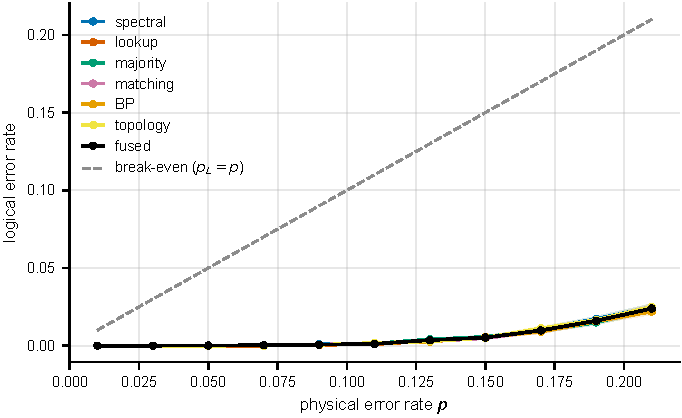
\includegraphics[width=0.72\textwidth]{fig_threshold.pdf}
    \caption{Logical error rate versus physical error rate $p$ for the core decoders on the repetition code under i.i.d.\ noise. All decoders track the optimal \texttt{lookup} leader closely and stay below the break-even line $p_L=p$; the curves overlap, consistent with the statistically indistinguishable logical error rates of Table~\ref{tab:main}. Lines are the mean logical error rate over $n=\sync{40{,}000}$ Monte-Carlo trials per point (reported scale) and shaded bands are analytic $95\%$ Bernoulli confidence intervals ($1.96\sqrt{\hat p(1-\hat p)/n}$); the bands overlap throughout. Generated from the run artifact \texttt{summary.json}.}
    \label{fig:threshold}
\end{figure}

\subsection{Selective decoding: abstention buys large, monotone reliability gains}
\label{sec:risk_coverage}

Because each decoder reports a confidence, we can let it \emph{abstain}: commit only on shots whose confidence exceeds a threshold, and sweep that threshold to trace a risk--coverage curve. Figure~\ref{fig:risk_coverage} shows the curves for the confidence-fused and matching decoders. The effect is large and monotone. At full coverage ($1.0$) the matching decoder has a pooled logical error of \sync{0.1529}; as its abstention threshold rises, coverage falls and committed risk drops sharply: to \sync{0.0757} at coverage \sync{0.545}---roughly a two-fold error reduction for committing to about half the shots---and to \sync{0.0099} at coverage \sync{0.247}, a more than fifteen-fold reduction for committing to roughly a quarter of the shots. The fused decoder traces a similarly favourable, monotone curve, reaching \sync{0.0499} risk at \sync{0.464} coverage and \sync{0.0101} at \sync{0.248} coverage. The monotonicity is verified programmatically by the runner.

The per-regime coverage values (Table~\ref{tab:main}, and Methods) make the mechanism concrete: matching abstains heavily under structured noise (coverage as low as \sync{0.28} under bias and \sync{0.50} under measurement error), pushing its errors onto the abstained shots, whereas majority, lookup, neural and fused always commit (coverage $1.0$) at the fixed operating threshold. This is exactly the selective-prediction trade-off~\cite{chow1970optimum,geifman2017selective}: a decoder that knows when it does not know is more valuable inside a fault-tolerant loop than one that is marginally more accurate but always commits. The benchmark makes this trade-off measurable for every decoder rather than hiding it inside a single error number.

\begin{figure}[htbp]
    \centering
    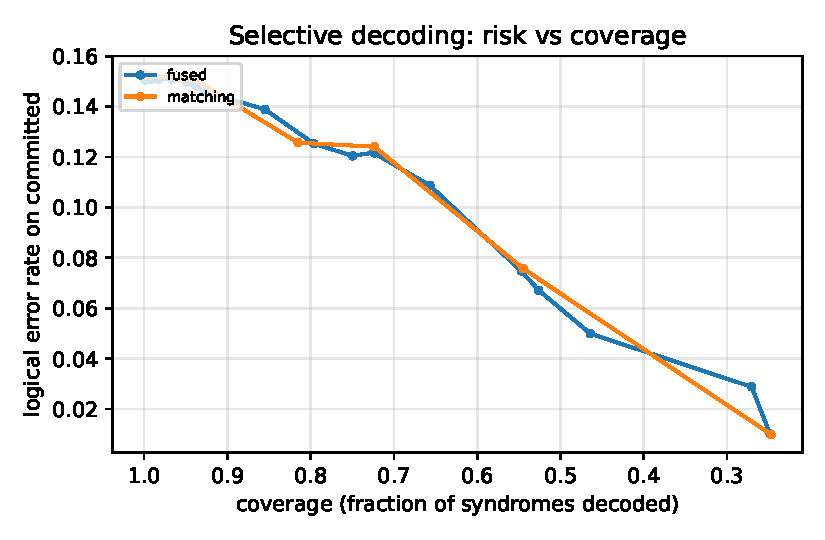
\includegraphics[width=0.72\textwidth]{fig_risk_coverage.pdf}
    \caption{Selective decoding. Risk (logical error rate on committed shots) versus coverage (fraction of syndromes decoded) for the fused and matching decoders, obtained by sweeping the abstention threshold (full coverage on the left). Risk falls monotonically as coverage shrinks: abstaining on low-confidence syndromes trades coverage for reliability. Lines are means over the $n=\sync{200{,}000}$ pooled shots per decoder (reported scale) and shaded bands are analytic $95\%$ Bernoulli confidence intervals of the committed error rate, whose effective sample size at each point is (coverage~$\times$~pooled shots). Generated from the run artifact \texttt{summary.json}.}
    \label{fig:risk_coverage}
\end{figure}

\subsection{Calibration is not predicted by decoder sophistication}
\label{sec:calibration}

The confidence that gates abstention is only useful if it is calibrated. The expected-calibration-error column of Table~\ref{tab:main} delivers the paper's most counterintuitive result: \emph{calibration is essentially uncorrelated with decoder sophistication, and not predictable from the logical error rate}. ECE ranges over a factor of eight across the family, in the order (best to worst): \texttt{neural} \sync{0.0317} $<$ \texttt{majority} \sync{0.0489} $<$ \texttt{lookup} \sync{0.0569} $<$ \texttt{fused} \sync{0.0608} $<$ \texttt{bp} \sync{0.1232} $<$ \texttt{rl} \sync{0.2387} $<$ \texttt{topology} \sync{0.2428} $<$ \texttt{matching} \sync{0.2608}. The best-calibrated decoder is the lightweight logistic-regression \texttt{neural} coset selector---by construction its confidence is a predicted-class probability, so it is approximately calibrated for the coset decision---while the \emph{worst}-calibrated decoder is plain minimum-weight \texttt{matching}, whose defect-fraction confidence heuristic tracks accuracy poorly. The two decoders that abstain most heavily (matching and topology) and the RL selector are the three worst calibrated, whereas three of the four always-covering decoders (neural, majority, lookup) are the three best.

\paragraph{A data-fidelity note.}
This ordering directly contradicts a natural intuition---and an explicit claim in the project's own README---that the confidence-\emph{fused} decoder is the best calibrated. It is not. At reported scale the fused decoder ranks fourth on ECE (\sync{0.0608}); the neural selector is best (\sync{0.0317}). (At the smaller smoke scale the ordering shifts again---there the \emph{majority} decoder is best calibrated, with fused third and neural fifth---which is itself a useful caution that small-sample calibration rankings are unstable.) We resolve the discrepancy in favour of the regenerated artifact: every ECE value in this paper is the value written to \texttt{summary.json} by the reported-scale run, and the narrative is built around those numbers rather than the prior claim. What survives across scales is the structural conclusion: calibration must be measured, not assumed from a decoder's accuracy or complexity. Among the always-covering decoders---where calibrated confidence is precisely what makes selective decoding usable---the fused decoder is still well calibrated (\sync{0.0608}) and noticeably better than belief propagation (\sync{0.1232}), but the lightweight neural classifier is better still; a deployment that needs trustworthy abstentions should prefer the explicitly probability-calibrated head. Treating calibration as a first-class metric is what makes any of this visible; optimising logical error rate alone would hide it entirely, since the eight decoders are tied on that axis.

\subsection{Structured noise separates regimes, not decoders}
\label{sec:per_regime}

The per-(regime, decoder) breakdown (Methods, Sec.~\ref{sec:methods_perregime}) confirms that the dominant axis of variation is the \emph{noise regime}, not the decoder. At reported scale the per-regime logical error rises from $\approx\sync{0.002}$ under i.i.d.\ noise to $\approx\sync{0.043}$ (biased), $\approx\sync{0.17}$ (burst), $\approx\sync{0.21}$ (correlated) and $\approx\sync{0.34}$ (measurement error) for essentially all decoders---a more than hundred-fold change driven entirely by structure, with the syndrome-read-out-noise regime by far the hardest. Within a regime the decoders again cluster within their (now tight) confidence intervals: under correlated noise \texttt{fused} reaches \sync{0.2062} and \texttt{topology} \sync{0.2078} against majority's \sync{0.2105}, and under measurement error \texttt{lookup} reaches \sync{0.3315} and \texttt{fused} \sync{0.3324} against majority's \sync{0.3401}---small, regime-dependent gaps that are at most marginally significant and are consistent with topology- or read-out-aware decoders helping slightly where structure exists. The integrity flag \texttt{automorphism\_invariant} is \sync{true}, confirming the matching decoder respects the code's cyclic symmetry to within statistical tolerance.

% ============================================================
\section{Discussion}
\label{sec:discussion}

\paragraph{What the benchmark establishes.}
The contribution of this work is methodological, not a new error rate. By placing eight decoders on one defect-graph interface and evaluating them across five structured-noise regimes with three metrics---logical error, calibration, and risk--coverage---each carrying explicit confidence intervals, the benchmark makes three things visible that a single-number i.i.d.\ comparison hides. First, on this code the decoders are statistically indistinguishable on raw logical error (a $\sync{0.0024}$ spread inside a $\approx\sync{0.0032}$ interval width); the honest conclusion is parity, not a winner. Second, abstention is a large and previously under-reported lever: committing to about a quarter of the shots cuts matching's committed logical error from \sync{0.1529} to \sync{0.0099}. Third, calibration is decoupled from both sophistication and accuracy---the eight decoders are tied on error rate yet span an eight-fold ECE range, and the best-calibrated decoder (the lightweight neural selector) is neither the most accurate nor the most elaborate. None of these is apparent without selectivity and calibration as primary axes.

\paragraph{Relation to prior work.}
Matching~\cite{dennis2002topological,fowler2012surface,higgott2022pymatching}, BP~\cite{poulin2008iterative,roffe2020decoding}, and neural/RL decoders~\cite{torlai2017neural,varsamopoulos2017decoding,sweke2020reinforcement,bausch2024learning} are each studied in depth, typically in isolation and under i.i.d.\ noise, and typically optimising logical error. Our framing is orthogonal: we import selective prediction~\cite{chow1970optimum,geifman2017selective,elyaniv2010foundations} and calibration~\cite{guo2017calibration} from machine learning and make them the evaluation lens for a whole decoder family under structured noise. We make no accuracy-superiority claim and, where the literature reports learned decoders exceeding matching on hardware syndromes~\cite{bausch2024learning}, we note that our toy-scale repetition code cannot and does not reproduce that regime; our purpose is the measurement methodology, not the record.

\subsection{Limitations}
\label{sec:limitations}
\begin{enumerate}[leftmargin=1.5em]
    \item \textbf{Toy codes only.} The primary benchmark is a one-dimensional repetition code; the second code is a surface-\emph{like} toy lattice, not a stabilizer-exact CSS surface code, and we do not evaluate a full surface code at scale. The repetition code corrects only bit-flip errors and has a trivial (line) defect geometry, which is part of why the decoders cluster so tightly.
    \item \textbf{Simulated structured noise.} All noise is produced by parametric samplers, not measured from hardware. The biased/burst/correlated/measurement-error regimes are plausible surrogates, but real device noise has correlations (leakage, crosstalk, drift) our samplers do not model.
    \item \textbf{Logical-error differences are within noise.} The decoders are statistically indistinguishable on raw logical error at the scales we ran; the benchmark's value is in selectivity and calibration, not in resolving an accuracy ranking. Larger codes and more shots would be needed to separate decoders on accuracy.
    \item \textbf{Single-distance focus.} The headline table is at one distance and one physical error rate; the threshold curves sweep $p$ at a fixed distance but we do not present a distance-scaling (sub-threshold) study, which is the decisive test for a true topological code.
    \item \textbf{Reduced-scope learned decoders.} The neural decoder is a logistic-regression coset selector and the RL decoder is a contextual bandit, not the deep graph or transformer decoders of the recent literature. Our calibration and selectivity findings are about these specific, lightweight models.
    \item \textbf{Solo author, single environment.} All results were produced and audited by one author on a single CPU platform; independent replication on other hardware and by other groups remains to be done.
\end{enumerate}

\paragraph{Conclusion.}
A deployable QEC decoder must do more than minimise an i.i.d.\ logical error rate: it must behave well under structured noise, know when to abstain, and report calibrated confidence. We built a reproducible benchmark that measures all three for a full decoder family on one defect-graph interface, and we report---honestly---that the decoders are statistically indistinguishable on raw logical error while differing sharply in calibration and in the reliability they buy through abstention. The most actionable findings are that abstention cuts committed logical error several-fold for a moderate coverage cost, and that the best-calibrated decoder is the simplest one, not the most elaborate. Extending the framework to a full surface code at scale, to hardware syndromes, and to a distance-scaling study---while keeping selectivity and calibration as first-class metrics---is the natural next step.

% ============================================================
\section{Methods}
\label{sec:methods}

\subsection{Codes}
\label{sec:methods_codes}
The repetition code (\texttt{RepetitionCode}) has $n=d$ data bits and $d-1$ weight-two checks $Z_iZ_{i+1}$; the syndrome of an error $e\in\F_2^d$ is $s_i=e_i\oplus e_{i+1}$. The logical observable is the global parity $\sum_i e_i \bmod 2$. A correction $\hat c$ is counted as a logical failure unless the residual $r=e\oplus\hat c$ has zero syndrome (is a stabilizer) and zero logical value; a residual that does not even reproduce the syndrome is also a failure. The lookup decoder enumerates all $2^d$ errors to tabulate the minimum-weight leader per syndrome. The surface-like code (\texttt{SurfaceLikeCode}) places $d^2$ data bits on a grid with $(d-1)^2$ plaquette (weight-four) checks; defects are paired by Manhattan-distance matching and the logical observable is the parity of the left column. Both codes expose a bipartite Tanner graph via \texttt{networkx}~\cite{hagberg2008exploring}.

\subsection{Structured-noise samplers}
\label{sec:methods_noise}
Each sampler takes a seeded \texttt{numpy} generator~\cite{harris2020array} and returns a $0/1$ error vector. \emph{i.i.d.}: each bit flips at rate $p$. \emph{biased}: even-index bits flip at $\min(1,\mathrm{bias}\cdot p)$ and odd-index bits at $p$ (default $\mathrm{bias}=3$). \emph{burst}: scanning the line, with probability $p$ a contiguous run of length $1+\mathrm{Poisson}(\mathrm{burst\_len}-1)$ is flipped (default $\mathrm{burst\_len}=3$). \emph{correlated}: an i.i.d.\ seed pattern recruits each neighbour with probability $\mathrm{corr}$ (default $0.5$) over two sweeps. \emph{measurement\_error}: i.i.d.\ data noise at rate $p$ plus a per-check syndrome-flip mask at rate $q$ (default $0.05$), which the runner XORs into the measured syndrome.

\subsection{Decoders}
\label{sec:methods_decoders}
Every decoder implements \texttt{decode(syndrome)$\to$(correction, confidence)}. \emph{Lookup}: table from syndrome to minimum-weight leader; confidence boosted toward $1$ since the leader is exact. \emph{Majority}: cumulative XOR of the syndrome recovers a flip chain up to a global offset, choosing the lower-weight coset representative; confidence is the normalised majority margin. \emph{Matching}: on the line, defects are paired left-to-right with boundary closure for an odd defect, returning the lighter coset; on the surface, a complete graph on lit plaquettes weighted by negative Manhattan distance is solved with \texttt{max\_weight\_matching}~\cite{edmonds1965paths,hagberg2008exploring} and an L-shaped path is flipped between matched pairs. Confidence is a defect-fraction heuristic $\exp(-2\,n_{\mathrm{def}}/n_{\mathrm{checks}})$, damped when a defect is unpaired. \emph{BP}: a few rounds of min-sum message passing on the Tanner graph with log-likelihood priors; if the thresholded beliefs do not reproduce the syndrome, it defers to matching. \emph{Neural}: a two-stage learned coset selector---a syndrome-determined base chain plus a \texttt{scikit-learn} logistic-regression classifier~\cite{pedregosa2011scikit} predicting the logical coset of the true correction relative to that chain; the output is always syndrome-consistent and confidence is the predicted-class probability. \emph{Topology}: matching with confidence recalibrated by defect-geometry features (count, span, gap structure). \emph{Fused}: matching and neural both propose; agreement boosts confidence, disagreement defers to the more confident proposal with damped confidence. \emph{RL}: a contextual bandit~\cite{li2010contextual,sutton2018reinforcement} whose context is a coarse defect-count bucket and whose actions are candidate decoders; it keeps per-context running success estimates, plays $\eps$-greedy during a warm-up stream, and at evaluation selects the highest-value decoder per context.

\subsection{Metrics and confidence intervals}
\label{sec:methods_metrics}
The logical error rate is the mean of per-shot failure indicators; its 95\% confidence interval is $1.96\,\hat\sigma/\sqrt n$ with $\hat\sigma$ the sample standard deviation (Bernoulli, so $\hat\sigma\approx\sqrt{\bar p(1-\bar p)}$). The expected calibration error~\cite{guo2017calibration,naeini2015obtaining} partitions shots into ten equal-width confidence bins and averages $\abs{\text{(mean confidence)}-\text{(mean accuracy)}}$ weighted by bin occupancy, where accuracy is $1-$failure. The risk--coverage curve sweeps an abstention threshold from the minimum to the maximum observed confidence; at each threshold, coverage is the committed fraction and risk is the logical error rate on committed shots. The curve is reported in descending-coverage order and a monotonicity check verifies that risk is (weakly) non-increasing as coverage shrinks.

\subsection{Integrity: automorphism invariance and the audit gate}
\label{sec:methods_audit}
The repetition code is invariant under cyclic relabeling of its data bits (ring symmetry); a faithful decoder must yield the same logical error rate on cyclically rotated errors. The runner checks this for the matching decoder over shifts $\{1,2,d/2\}$ within a statistical tolerance and exposes it as the \texttt{automorphism\_invariant} flag. A separate audit module enforces that every reported number traces to a value in the generated \texttt{summary.json} (the single source of truth) and rejects forbidden absolute-superiority phrasing; this discipline is run in continuous integration.

\subsection{Experimental protocol}
\label{sec:methods_protocol}
A run builds the code, fits the neural decoder on a mixed-regime training stream, warms up the RL bandit on its own Monte-Carlo stream, then for each (regime, decoder) Monte-Carlos \texttt{trials} shots at the evaluation physical error rate $p_{\mathrm{eval}}$, records the per-shot failure/confidence, and aggregates the metrics above. Threshold curves sweep $p$ for the core decoders under i.i.d.\ noise; the risk--coverage curve is built from the fused and matching decoders' pooled confidences. Seeds, platform, library versions, runtime and peak memory are recorded as provenance in \texttt{summary.json}. All numbers in this paper are from the \emph{reported-scale} configuration: distance $\sync{9}$, $\sync{40{,}000}$ trials per (regime, decoder) ($\sync{200{,}000}$ pooled shots per decoder), $\sync{20{,}000}$ training shots, $p_{\mathrm{eval}}=\sync{0.12}$, an eleven-point physical-error grid, run end-to-end in $\sync{507}$\,s at $\sync{200}$\,MB peak memory on a single CPU. A faster smoke configuration (distance $\sync{5}$, $\sync{1{,}500}$ trials, $\approx\sync{13}$\,s) is provided for continuous integration. Software: \texttt{numpy}~\cite{harris2020array}, \texttt{scipy}~\cite{virtanen2020scipy}, \texttt{networkx}~\cite{hagberg2008exploring}, \texttt{scikit-learn}~\cite{pedregosa2011scikit}, \texttt{matplotlib}~\cite{hunter2007matplotlib}; CPU only.

\subsection{Per-regime results}
\label{sec:methods_perregime}
The per-(regime, decoder) logical error rate, ECE and coverage at $p_{\mathrm{eval}}$ are written in full to \texttt{summary.json} under \texttt{by\_regime}. At reported scale the qualitative pattern is regime-dominated: i.i.d.\ noise yields $\approx\sync{0.002}$ logical error across decoders; biased $\approx\sync{0.043}$; burst $\approx\sync{0.17}$; correlated $\approx\sync{0.21}$; measurement-error $\approx\sync{0.34}$ (the hardest regime, since syndrome read-out flips corrupt the very signal the decoders condition on). Within each regime the decoders cluster within their confidence intervals, while coverage varies strongly by decoder: matching's coverage at the fixed operating threshold ranges from \sync{0.28} (biased) to \sync{0.67} (i.i.d.); topology and the RL selector also abstain substantially; majority, lookup, neural and fused commit fully (coverage $1.0$) in every regime.

% ============================================================
\section*{Data availability}
This study uses no external datasets. All numerical values, tables, and figures are generated by the accompanying scripts from fixed random seeds and are written to a single source-of-truth artifact (\texttt{results/summary.json}); they are reproduced by running the pipeline.

\section*{Code availability}
The code that implements every code, noise model, decoder, metric, and the audit gate, and that regenerates every figure, table, and reported number, accompanies this manuscript in \texttt{submission/code} and is intended for public release upon publication.

\section*{Competing interests}
The author declares no competing interests.

\section*{Author contributions}
M.H. conceived the study, designed and implemented the benchmark, decoders, noise models, metrics and audit pipeline, ran and analysed the experiments, and wrote the manuscript.

\section*{Funding}
The author received no specific funding for this work.

\section*{Reproducibility statement}
All experiments are reproducible on commodity hardware; runtime and memory are reported for each benchmark.

% ============================================================
\bibliographystyle{unsrtnat}
\bibliography{refs}

\end{document}
